\documentclass[11pt,a4paper]{report}

\usepackage[a4paper,margin=2.5cm]{geometry}
\usepackage[utf8]{inputenc}
\usepackage[T1]{fontenc}
\usepackage{graphicx}
\usepackage{xcolor}
\usepackage{booktabs}
\usepackage{longtable}
\usepackage{array}
\usepackage{enumitem}
\usepackage{fancyhdr}
\usepackage{titlesec}
\usepackage{listings}
\usepackage[colorlinks=true,linkcolor=blue!50!black,urlcolor=blue!50!black,citecolor=blue!50!black]{hyperref}
\usepackage{parskip}
\usepackage{tabularx}

\definecolor{codebg}{RGB}{245,245,245}
\lstset{
  basicstyle=\ttfamily\footnotesize,
  backgroundcolor=\color{codebg},
  frame=single,
  breaklines=true,
  columns=fullflexible,
  keepspaces=true,
  numbers=none,
  showstringspaces=false
}

\pagestyle{fancy}
\fancyhf{}
\fancyhead[L]{Strata --- Multi-Site IaaS Infrastructure}
\fancyhead[R]{\thepage}
\renewcommand{\headrulewidth}{0.4pt}

\titleformat{\chapter}[hang]{\normalfont\Huge\bfseries}{\thechapter.}{20pt}{\Huge}

\title{
  \Large University of Algiers 1 --- M1 RSE \\[1em]
  \Huge\bfseries Strata \\[0.3em]
  \Large Design and Deployment of a Multi-Site IaaS Provider Infrastructure \\[1em]
  \large Network, Systems and Platform Engineering Report
}
\author{Derar Chekrouni}
\date{2026}

\begin{document}

\maketitle

\begin{abstract}
\noindent
This report documents the design and deployment of the network and systems
infrastructure for Strata, a fictional multi-site Infrastructure-as-a-Service
(IaaS) provider built as part of the M1-RSE ``Deployment and Security
Evaluation of a Multi-Site IaaS Cloud Provider Infrastructure'' project. It
covers the two-site architecture (a corporate Headquarters and a Cloud
Datacenter), the network design and redundancy mechanisms used at each layer,
the perimeter and inter-site security design, the core infrastructure
services, database high availability, the automation layer, and the two
web applications built on top of this infrastructure. Intrusion detection
and the controlled attack-simulation campaign were carried out by a
teammate and are documented separately; they are out of scope here.
\end{abstract}

\tableofcontents

% =====================================================================
\chapter{Introduction and Project Context}
% =====================================================================

Strata is a fictional Infrastructure-as-a-Service (IaaS) provider that, like
any real cloud operator, must run its own corporate operations while
simultaneously hosting and exposing compute resources sold to external
customers. This dual nature --- an internal enterprise network alongside a
customer-facing public cloud --- is the central design constraint of the
project: the two populations, internal staff and external customers, must be
strictly separated at every layer, while both are still served by a coherent,
centrally managed and automated infrastructure.

Strata's infrastructure is split across two physically distinct sites,
interconnected over an untrusted ISP transit:

\begin{itemize}[leftmargin=1.5em]
  \item \textbf{Headquarters (HQ)} hosts Strata's internal corporate network
    and the operational systems used by its \textasciitilde20 staff, organized
    into an IT department (Engineering, Operations, Support teams), HR, and
    Management.
  \item \textbf{Cloud Datacenter} hosts the customer-facing IaaS
    infrastructure: the compute fabric, the customer portal, and the
    workloads consumed by external customers.
\end{itemize}

This report covers the work carried out on the network, systems, automation,
and application layers of this infrastructure. The intrusion-detection
layer and the seven mandatory attack-simulation scenarios required by the
project brief were the responsibility of a teammate and are documented in a
separate report.

% =====================================================================
\chapter{Architecture Overview}
% =====================================================================

\section{Site layout}

The two sites connect to the public internet through their own,
independent ISP links, and to each other through a site-to-site
interconnection terminated at each site's perimeter gateway (Chapter
\ref{ch:interconnect}). Figures \ref{fig:brancha} and \ref{fig:branchb} show
the as-built topology of each site.

\begin{figure}[htbp]
  \centering
  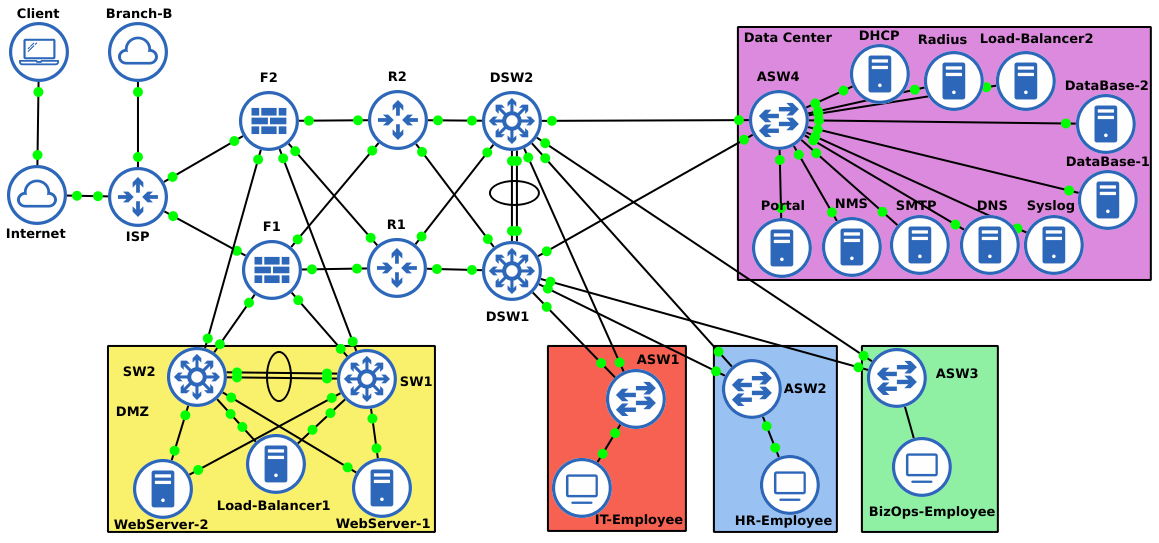
\includegraphics[width=0.95\textwidth]{Architecture/Branch A.png}
  \caption{Headquarters (Branch A) --- redundant three-tier campus design.}
  \label{fig:brancha}
\end{figure}

\begin{figure}[htbp]
  \centering
  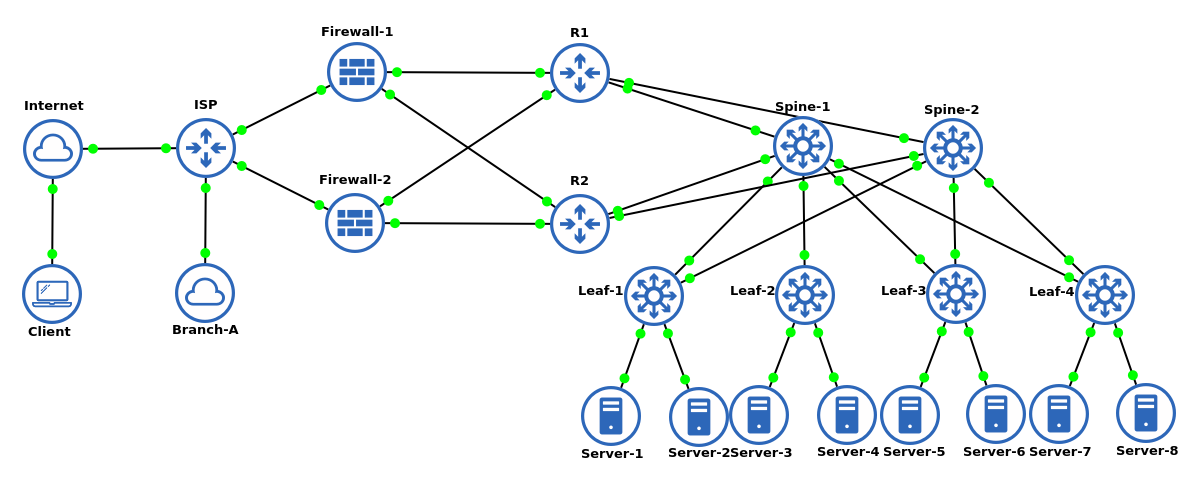
\includegraphics[width=0.95\textwidth]{Architecture/Branch B.png}
  \caption{Cloud Datacenter (Branch B) --- spine-leaf compute fabric.}
  \label{fig:branchb}
\end{figure}

\textbf{Headquarters} follows a classic redundant three-tier enterprise
design: a dual-firewall perimeter (F1/F2), a dual-router core (R1/R2), a
dual distribution-switch layer (DSW1/DSW2), and an access layer split by
department (IT/HR/BizOps), plus a DMZ hosting the employee-facing web tier
and a Data Center segment hosting shared internal services (DHCP, RADIUS,
mail, DNS, monitoring, load balancing, databases). Every tier above the
access layer is built as a redundant pair with full-mesh links between
adjacent tiers, so that no single link or device failure isolates a zone.

\textbf{Cloud Datacenter} is built around a spine-leaf Clos fabric behind
its own redundant firewall/router pair: two spine switches form the fabric
core with no direct spine-to-spine link, and each leaf switch connects to
every spine, giving any two leaves at least two independent paths between
them. Customer workload hosts (VMs and containers) attach to the leaves.

\section{Network segmentation}

Both sites enforce a mandatory zone model, with all inter-zone traffic
passing through a stateful firewall:

\begin{itemize}[leftmargin=1.5em]
  \item \textbf{Public / DMZ zone} (Datacenter) --- the externally reachable
    layer hosting the customer portal and its API. Treated as hostile
    territory: a compromise here must not grant access to customer
    workloads, the database tier, or HQ.
  \item \textbf{Customer workload zone} (Datacenter) --- the spine-leaf
    fabric hosting customer compute. Reachable from the DMZ only for the
    strict minimum traffic required by the provisioning control plane.
  \item \textbf{Internal corporate network} (HQ) --- accessible exclusively
    to Strata staff, hosting the employee portal and directory service. No
    path exists from the Datacenter DMZ into this zone.
  \item \textbf{Backend data zone} --- the replicated database tier,
    unreachable from the DMZ; only the appropriate application servers may
    connect to it.
\end{itemize}

An explicit, documented zone-to-zone policy governs every permitted flow
(Section \ref{sec:aclpolicy}); everything else is denied by default at the
gateway.

% =====================================================================
\chapter{Network Design}
% =====================================================================

\section{Addressing plan}

The whole internal address space is drawn from \texttt{10.0.0.0/16},
fully documented interface-by-interface and device-by-device in
\texttt{Adressing/} (\emph{IPv4 Addresses.pdf}, \emph{Connections.pdf}).
Summary:

\begin{table}[htbp]
\centering
\begin{tabular}{llll}
\toprule
VLAN & Purpose & Subnet & Gateway (HSRP VIP) \\
\midrule
90  & Management & 10.0.9.0/28  & 10.0.9.1 \\
100 & IT         & 10.0.10.0/28 & 10.0.10.1 \\
200 & HR         & 10.0.20.0/28 & 10.0.20.1 \\
300 & BizOps     & 10.0.30.0/28 & 10.0.30.1 \\
400 & Data Center& 10.0.40.0/28 & 10.0.40.1 \\
10  & DMZ        & 10.0.1.0/29  & 10.0.1.1 \\
\bottomrule
\end{tabular}
\caption{HQ VLAN addressing plan.}
\end{table}

Every point-to-point inter-device link (firewall--router, router--switch,
spine--leaf, etc.) is allocated its own /30, and every device carries a
/32 loopback used as its OSPF router-id and management identity. One public
IPv4 (\texttt{203.0.113.8/32}) is reserved for the DMZ load balancer.

\section{Routing}

OSPF runs throughout, area 0 at HQ and area 1 across the Datacenter fabric,
with every inter-device link tuned as \texttt{point-to-point} to avoid
unnecessary DR/BDR election overhead on links that only ever have two
neighbors. Example, from a core router:

\begin{lstlisting}
router ospf 1
 passive-interface Loopback0
 network 10.0.0.3 0.0.0.0 area 0
\end{lstlisting}

Firewalls originate a default route toward the ISP; everything else is
learned dynamically, so a new device or a new redundant path only needs an
OSPF adjacency, not a manual static-route update anywhere else in the
fabric.

\section{Redundancy design}

Redundancy was treated as a first-class design constraint from the start,
organized around three axes:

\begin{itemize}[leftmargin=1.5em]
  \item \textbf{Hardware / link redundancy} --- LACP EtherChannel bundles
    (\texttt{channel-group 1 mode active}) between the DSW1/DSW2 pair and
    between the DMZ switch pair, so a single physical link failure between
    either pair has zero impact.
  \item \textbf{Network / path redundancy} --- HSRP active/standby gateways
    on every VLAN SVI at HQ, and ECMP across the spine-leaf fabric in the
    Datacenter.
  \item \textbf{Data redundancy} --- Patroni-managed PostgreSQL
    primary/replica replication for both application databases
    (Chapter \ref{ch:db}).
\end{itemize}

HSRP is deliberately load-shared rather than pinned to a single active
switch: DSW1 is HSRP-active (and DSW2 standby) for VLANs 90/100/200, while
the priorities are reversed for VLANs 300/400, so that under normal
conditions both distribution switches are forwarding traffic rather than
one sitting idle. Example HSRP/VLAN block:

\begin{lstlisting}
interface Vlan 100
 ip address 10.0.10.2 255.255.255.240
 ip helper-address 10.0.40.2
 standby 10 ip 10.0.10.1
 standby priority 110
 standby preempt
\end{lstlisting}

\section{Spine-leaf compute fabric}

The Datacenter's customer-workload network follows the standard Clos
topology mandated by the project brief: two spines, no direct
spine-to-spine link, and every leaf connected to every spine so that ECMP
distributes traffic across both spine uplinks and the loss of a single
spine does not partition any pair of leaves. The fabric is implemented as a
Containerlab topology (\texttt{Automation/} \textrightarrow{}
\texttt{Config/Devices/Containerlab/Branch-B.yml}): the core router is
Cisco IOL (IOS-on-Linux), spine and leaf are Arista cEOS, each running OSPF
with router-ids matching the addressing plan. The leaf's server-facing
interface relays DHCP to the Data Center DHCP server, exactly as the
physical-VM build does at HQ:

\begin{lstlisting}
interface Ethernet2
 ip address 10.10.10.1/24
 ip helper-address 10.0.40.2
 no switchport
 router ospf 1
  router-id 10.0.0.8
  area 0.0.0.1
\end{lstlisting}

Building this fabric as containers rather than full VMs (as the rest of the
HQ lab is built) keeps the Datacenter side lightweight enough to run
alongside the customer-workload VMs/containers it hosts on the same
hypervisor, while still exercising the same routing behaviour as the
physical build.

% =====================================================================
\chapter{Perimeter Security and Site Interconnection}
\label{ch:interconnect}
% =====================================================================

\section{Gateway and firewall design}

Both sites' perimeters are pfSense firewalls, each acting as the dedicated
gateway for every inter-zone flow at that site: routing between the
external network, the local zones, and the inter-site link; stateful,
default-deny firewall rules between every zone pair; NAT for outbound
traffic and inbound access to published services; and logging of denied
flows for later reconstruction.

\subsection{Zone-to-zone policy}
\label{sec:aclpolicy}

The access policy actually implemented (translated into pfSense firewall
rules at the relevant interfaces) is:

\begin{itemize}[leftmargin=1.5em]
  \item Only IT staff may reach the Data Center zone (full access within it).
  \item Every department gets access to the internal web portal
    (HTTPS/443) only.
  \item DHCP (67) and DNS (53) are permitted where required for client
    bootstrap.
  \item The DMZ web server may reach the internal database only on
    PostgreSQL/5432 --- nothing else.
  \item No external client has any path into the internal network.
  \item Only the IT department may reach the branch office link.
  \item Traffic from the DMZ/Data Center toward the branch office is
    limited to the strict minimum necessary.
\end{itemize}

This is a default-deny policy with a short, explicit allow-list --- every
permitted flow above corresponds to a concrete pfSense rule scoped to a
specific interface, protocol, and destination, rather than a broad
zone-to-zone allow.

\section{Site-to-site interconnection}

Branch sites are interconnected over an Ethernet WAN service provided by
the ISP. Because that transit infrastructure is outside organizational
control, a site-to-site IPsec VPN is deployed between the two sites'
perimeter firewalls to guarantee confidentiality, integrity, and
authentication of all inter-site traffic. The tunnel terminates directly at
each site's gateway, so a tunnel failure simply removes the inter-site path
rather than exposing anything in plaintext, and firewall rules are enforced
at both tunnel endpoints so only the traffic explicitly permitted by the
zone policy above ever crosses it.

% =====================================================================
\chapter{Core Infrastructure Services}
% =====================================================================

All core services run in the HQ Data Center zone and are reachable by the
rest of the internal network only on the ports they need. Software choices
are summarized in Table \ref{tab:software}.

\begin{table}[htbp]
\centering
\begin{tabular}{ll}
\toprule
Function & Software \\
\midrule
DHCP & ISC \texttt{dhcpd} \\
DNS & ISC BIND9 \\
AAA / RADIUS & FreeRADIUS + PostgreSQL \\
SMTP & Postfix \\
IMAP & Dovecot \\
SNMP / metrics & LibreNMS \\
Centralized logging & Graylog (MongoDB-backed) \\
Config management & Ansible \\
Compute provisioning & Terraform (libvirt, Docker) \\
\bottomrule
\end{tabular}
\caption{Core software stack.}
\label{tab:software}
\end{table}

\section{DHCP and dynamic DNS}

\texttt{dhcpd} serves one pool per VLAN (e.g. \texttt{10.0.10.4}--\texttt{10.0.10.14}
for IT, 600 s default / 7200 s max lease), handing out the HSRP VIP of the
relevant VLAN as the default gateway. Every lease triggers a secure Dynamic
DNS update to BIND, authenticated with a TSIG key (HMAC-SHA256) so that
only the DHCP server can write records into the zone:

\begin{lstlisting}
key dhcp-key {
    algorithm hmac-sha256;
    secret "<redacted>";
};
zone "pfe2627.xyz" {
    type master;
    allow-update { key dhcp-key; };
};
\end{lstlisting}

Four matching reverse zones (one per VLAN subnet) keep PTR records in sync
the same way, so every dynamically leased address is both forward- and
reverse-resolvable without any manual DNS maintenance. In the Cloud
Datacenter, DHCP additionally drives the NAT-automation pipeline described
in Chapter \ref{ch:cloud} --- an \texttt{on commit} hook fires for every
lease to allocate and install a public-IP mapping for the new workload.

\section{AAA}

FreeRADIUS is backed by a PostgreSQL database rather than flat files, so
authentication and accounting records are queryable and centrally managed.
Connection limits are capped (\texttt{max\_connections = 16},
\texttt{idle\_timeout = 30}) to bound resource usage from any single NAS
client.

\section{Mail}

Postfix and Dovecot together provide internal-plus-external mail: Postfix
handles virtual mailbox routing for the \texttt{pfe2627.xyz} domain
(a dedicated \texttt{vmail} system account, uid/gid 5000) and relays
outbound mail through an authenticated, TLS-enforced external relay;
inbound submission (port 587) requires SASL authentication, which Postfix
delegates to Dovecot over a Unix socket rather than implementing its own
auth backend. Dovecot stores mail as Maildir, one directory tree per
domain/user, and exposes both IMAP and IMAPS.

\section{Monitoring and centralized logging}

LibreNMS (behind an nginx/PHP-FPM front end) provides SNMP-based device and
service monitoring across both sites. Every network device and service host
is configured (via the Ansible \texttt{syslog.yml} playbook) to ship its
logs to a single Graylog instance, which journals and indexes them in
MongoDB and exposes a single searchable interface --- filterable by time
range, source, and severity --- instead of requiring an operator to log
into each device individually to investigate an incident.

% =====================================================================
\chapter{Database Layer: PostgreSQL High Availability}
\label{ch:db}
% =====================================================================

Both application databases --- the Cloud platform's backend database and
the internal Employee Portal's database --- are deployed in a
\textbf{Patroni-managed primary/replica} configuration rather than a bare
single-instance PostgreSQL server, satisfying the project's requirement
that the database tier tolerate the loss of its primary node without losing
committed data or requiring lengthy manual intervention.

Patroni is a template for PostgreSQL HA that does not itself replicate
data; it orchestrates PostgreSQL's own native streaming replication and
adds automatic leader election and failover on top of it:

\begin{itemize}[leftmargin=1.5em]
  \item Each PostgreSQL node runs alongside a local Patroni agent, which
    exposes a REST API used for health checks and for the load
    balancer/proxy layer to always route writes to the current leader.
  \item Cluster state and leader election are coordinated through a
    distributed configuration store (DCS) --- etcd in this deployment ---
    which all Patroni agents watch. The DCS, not PostgreSQL itself, is the
    source of truth for \emph{who is currently primary}.
  \item Replicas stream changes from the primary via PostgreSQL's built-in
    streaming replication (WAL shipping), continuously staying within a
    small replication lag of the primary under normal load.
  \item If the primary becomes unreachable, Patroni's agents detect the
    loss of its DCS lease, hold a new leader election among the surviving
    replicas, and promote the most up-to-date one to primary automatically
    --- no operator action required to resume write availability.
  \item Periodic base backups (e.g. via \texttt{pg\_basebackup}/WAL
    archiving) are retained independently of the replication stream, so
    that recovery remains possible even in the event of a
    cluster-wide failure, not just a single-node one.
\end{itemize}

This design directly follows the standard Patroni HA-plus-backup pattern
for PostgreSQL, as described for example in
\url{https://medium.com/@yaseminbsra.sergen/postgresql-with-patroni-high-availability-and-backup-integration-1fd97bffbac1}.
Applying it to both databases means neither the customer-facing Cloud
platform nor the internal Portal has a single PostgreSQL instance as a
single point of failure --- consistent with the redundancy philosophy
applied at every other layer of this infrastructure (Section
\ref{sec:aclpolicy} and Chapter 3).

% =====================================================================
\chapter{Automation}
% =====================================================================

The project deliberately started from a traditionally, manually configured
infrastructure and evolved toward an automated one, so that the automation
layer reflects a real operational workflow rather than a from-scratch
Infrastructure-as-Code exercise.

\section{Ansible --- configuration management}

Inventory is grouped by role (\texttt{Routers}, \texttt{Switches},
\texttt{AccessSwitches}, and their \texttt{NetworkDevices} parent group;
\texttt{Servers} separately), with group-scoped connection variables
(\texttt{network\_cli}/\texttt{ios} for network devices, plain SSH for
servers) and vaulted (AES-256 encrypted) credentials per group. Playbooks
in production use:

\begin{itemize}[leftmargin=1.5em]
  \item \texttt{global\_conf.yml} --- console/VTY session hygiene
    (\texttt{exec-timeout 30}, synchronous logging) and a shared DNS
    resolver, pushed to every network device.
  \item \texttt{ntp.yml} --- NTP server and timezone, with a verification
    step against \texttt{show ntp associations}.
  \item \texttt{snmp.yml} --- SNMP read-only community, verified against
    \texttt{show snmp community}.
  \item \texttt{stp\_feat.yml} --- Rapid-PVST globally, \texttt{portfast}
    and \texttt{bpduguard} on access-layer edge ports.
  \item \texttt{syslog.yml} --- points every device at the central Graylog
    instance and enables debug-level trap logging.
  \item \texttt{package\_install.yml} --- baseline provisioning of the
    web-application hosts (nginx, Node.js 20.x, npm, pm2).
\end{itemize}

\section{Terraform --- self-service compute provisioning}

Terraform underpins the Cloud platform's self-service compute layer,
provisioning both of its compute tiers:

\begin{itemize}[leftmargin=1.5em]
  \item \texttt{VPS.tf} / \texttt{cloudinit.tf} --- KVM virtual machines
    via the \texttt{dmacvicar/libvirt} provider (SSH-connected to the
    hypervisor), each tenant getting its own libvirt storage pool, a
    cloud-init-driven first boot (user creation, SSH key injection,
    package installation), and a serial console exposed for remote
    troubleshooting.
  \item \texttt{Container.tf} --- Docker containers via the
    \texttt{kreuzwerker/docker} provider (over the same SSH transport to
    the hypervisor), tagged per tenant, as the lighter-weight compute tier
    of the same platform.
\end{itemize}

Both templates are invoked directly by the Cloud platform's backend on
every customer VM/container creation request (Chapter \ref{ch:cloud}),
turning what would otherwise be manual hypervisor administration into an
API-driven, self-service workflow --- the core requirement of an IaaS
offering.

% =====================================================================
\chapter{Application Layer}
% =====================================================================

Two applications run on top of this infrastructure, one per site, matching
the strict population separation required by the project brief: an
external, customer-facing platform in the Datacenter DMZ, and an internal,
staff-only portal at HQ that is not reachable from the DMZ at all.

\section{Cloud platform (Datacenter DMZ)}
\label{ch:cloud}

The customer-facing IaaS portal lets customers sign up, provision and
manage compute resources, and reach them once running. Concretely, it
provides:

\begin{itemize}[leftmargin=1.5em]
  \item \textbf{Self-service provisioning} of VMs (multiple official cloud
    images, plus a validated bring-your-own-image option restricted to an
    allow-listed set of official distribution mirrors) and containers,
    backed directly by the Terraform templates in Chapter 6.
  \item \textbf{Lifecycle control} --- start/stop/reboot, with the backend
    reconciling the platform's own state against the real hypervisor state
    on every request rather than trusting an optimistic write, so the UI
    never drifts out of sync with what is actually running.
  \item \textbf{A real in-browser console}, bridging the browser to the
    VM's serial console over a WebSocket relay, so a customer can reach a
    VM even before or without any network path being fully configured.
  \item \textbf{Live resource metrics} (CPU, memory, disk, network) sourced
    from the guest agent running inside each VM.
  \item \textbf{Public reachability} for every provisioned VM through the
    Datacenter's dedicated NAT gateway: each VM's private address is
    automatically mapped to a public address from a dedicated pool the
    moment DHCP assigns it a lease, and unmapped automatically when the VM
    is destroyed, requiring no manual network administration per customer
    workload.
\end{itemize}

Custom-image downloads are content-addressed and cached on the hypervisor:
the same image URL, requested by any customer, is downloaded once and
reused for every subsequent VM built from it, rather than re-fetched per
VM.

\section{Employee Portal (HQ, internal only)}

The internal portal is the single application through which Strata's staff
conduct all internal work, authenticated against a centralized directory
service and gated by department/role. It provides internal mail (with
attachments backed by the shared file repository), a file-sharing
repository with directory-level access permissions by department, an IT
helpdesk ticketing interface routed to the Support team, an HR
self-service module (leave requests, payslips, HR documents), a
cloud-operations dashboard giving Operations/Engineering a real-time view
of the Datacenter fabric and platform health, and a company/department
announcement board for Management.

% =====================================================================
\chapter{Lessons Learned and Future Work}
% =====================================================================

The project deliberately progressed through successive tooling phases
rather than being built once end-to-end: an initial single-firewall,
single-router design (still visible in the earliest addressing
documentation) was replaced by the fully redundant dual-firewall/
dual-router/dual-distribution-switch design once the cost of asymmetric
redundancy became clear; the network build itself moved from Packet
Tracer, to a full GNS3/EVE-style VM lab for maximum platform fidelity, to a
Containerlab-based container implementation of the Datacenter fabric once
running full router/switch VMs alongside dozens of customer VMs became
impractical on a single hypervisor.

Outstanding items, tracked for future iterations of this infrastructure:

\begin{itemize}[leftmargin=1.5em]
  \item Layer-2 edge hardening beyond what is already deployed
    (Port Security, DHCP Snooping, Dynamic ARP Inspection), intentionally
    sequenced last since it depends on every access-layer VLAN/port
    assignment being finalized first.
  \item Full alignment with the standard cloud-computing service
    characteristics (on-demand self-service, broad network access,
    resource pooling, rapid elasticity, measured service) --- most are
    already met by the Terraform-driven provisioning layer; measured
    service (usage-based accounting) is the remaining gap.
  \item Customer VPS disk encryption at rest (LUKS), with the encryption
    key held by the customer rather than the platform operator.
\end{itemize}

% =====================================================================
\chapter{Conclusion}
% =====================================================================

This report has covered the design and deployment of Strata's network and
systems infrastructure across two sites: a redundant enterprise campus at
Headquarters and a spine-leaf compute fabric in the Cloud Datacenter,
interconnected over an authenticated, encrypted site-to-site link, with a
strict, explicit, default-deny zone policy enforced at every boundary. On
top of this network, a full set of core infrastructure services (DHCP/DNS,
AAA, mail, monitoring, centralized logging) was deployed and largely
automated through Ansible, a highly-available PostgreSQL database layer was
built for both applications running on the platform, and a Terraform-driven
self-service compute layer turns the Datacenter fabric into an actual,
usable IaaS offering with real customer-facing provisioning, lifecycle
management, console access, and public reachability. Together with the
internal Employee Portal, this constitutes the full network-and-systems
half of the Strata project, with the intrusion-detection and attack
resilience evaluation carried out separately by a teammate as the
project's other half.

\end{document}
